\chapter{Выбор параметров нелинейных моделей}

%%%%%%%%%%%%%%%%%%%%%%%%%%%%%%%%%%%%%%%%%%%%%%%%
\section{Задача оптимизации}
%%%%%%%%%%%%%%%%%%%%%%%%%%%%%%%%%%%%%%%%%%%%%%%%

Модель $f( \bx, \bw)$ с параметрами $\bw \in \mathbb{R}^p$ предсказывает целевую переменную~$y \in \bbY$ по объекту~$\bx \in \bbR^{n}$. Пространство~$\bbY$ представляет собой бинарные метки классов~$\{0, 1\}$ для задачи двухклассовой классификации и~$\bbR$ для задачи регрессии.
Даны матрица плана~$\bX = [\bx_1, \dots, \bx_m]^{\T} \in \bbR^{m \times n}$ и целевой вектор~$\by = [y_1, \dots, y_m]^{\T} \in \bbY^{m}$. 
Цель состоит в нахождении оптимальных параметров~$\bw^*$.
Параметры~$\bw$ вычисляются минимизацией функции ошибки:
\begin{equation}
\bw^* = \argmin_{\bw \in \bbR^p} \cL(\bw, \bX, \by, f).
\label{eq:error_function}
\end{equation}
В качестве функции ошибки~$\cL (\bw, \bX, \by, f)$ рассматриваются квадратичная ошибка для задачи регрессии:
\begin{equation}
\cL(\bw, \bX, \by, f) = \frac 12 \| \by - \mathbf{f}(\bX, \bw) \|_2^2 = \frac 12 \sum_{i=1}^m \bigl( y_i - f(\bx_i,  \bw)\bigr)^2,
\label{eq:squared_error}
\end{equation}
и функция кросс-энтропии для задачи бинарной классификации: 
\begin{equation}
\cL(\bw, \bX, \by, f) = \sum_{i=1}^m \bigl[y_i \log f (\bx_i , \bw) + (1-y_i) \log \bigl(1 - f (\bx_i , \bw)\bigr)\bigr].
\label{eq:log_loss}
\end{equation}

Задача~\eqref{eq:error_function} решается с помощью итеративной процедуры оптимизации. 
Для получения параметров на шаге~$k$ текущие параметры $\bw^{k-1}$ обновляются по следующему правилу:
\begin{equation}
\bw^k = \bw^{k - 1} + \Delta \bw^{k - 1}.
\label{eq:update_rule}
\end{equation}
Авторы используют метод оптимизации Ньютона для выбора вектора обновлений~$\Delta \bw$.

Метод Ньютона нестабилен и вычислительно сложен. 
В данной статье предлагается стабильный алгоритм Ньютона. 
Перед шагом градиента предлагается выбрать подмножество активных параметров модели, которые оказывают наибольшее влияние на функцию ошибки~$\cL (\bw, \bX, \by, f)$.
Обновление параметров производится только для отобранного множества индексов~$\cA = \{j: a_j = 1, \ba \in \{0, 1\}^p\}$

\begin{align*}
\bw_{\cA}^k &= \bw_{\cA}^{k - 1} + \Delta \bw_{\cA}^{k - 1}, \quad \bw_{\cA} = \{w_j: j \in \cA \}; \\
\bw_{\bar{\cA}}^k &= \bw_{\bar{\cA}}^{k - 1}, \quad \bw_{\bar{\cA}} = \{w_j: j \notin \cA \}.
\end{align*}
Чтобы выбрать оптимальное подмножество индексов~$\cA$, из всех возможных $2^p - 1$~подмножеств, вводится функция ошибки
\begin{equation}
\ba = \argmin_{\ba' \in \{0, 1\}^p} S(\ba', \bX, \by, f, \bw),
\label{eq:subset_selection}
\end{equation}
аналогичная функции ошибки~\eqref{eq:feature_selection} для задачи выбора признаков. 
Задача~\eqref{eq:subset_selection} решается на каждом шаге $k$ процесса оптимизации для текущих параметров~$\bw^k$.

Алгоритм QPFS используется для решения задачи~\eqref{eq:subset_selection}.
QPFS выбирает подмножество параметров~$\ba$ для вектора обновлений~$ \Delta \bw$, которые оказывают наибольшее влияние на вектор остатков и являются попарно независимыми.
Функция ошибки~\eqref{eq:qpfs_problem} соответствует функции ошибки~$S(\ba, \bX, \by, f, \bw)$
\begin{equation}
\ba = \argmax_{\ba' \in \{1, 0\}^p} S(\ba', \bX, \by, f, \bw) \Leftrightarrow \argmin_{\ba  \in \bbR^p_+, \, \|\ba\|_1=1} \bigl[\ba^{\T} \bQ \ba - \alpha \cdot \mathbf{b}^{\T} \ba \bigr].
\end{equation}
В работе показано, что для модели нелинейной регрессии с квадратичной функцией ошибки~\eqref{eq:squared_error} и для модели логистической регрессии с кросс-энтропией~\eqref{eq:log_loss}, каждый шаг оптимизации эквивалентен задаче линейной регрессии~\eqref{eq:linear_regression}.



%%%%%%%%%%%%%%%%%%%%%%%%%%%%%%%%%%%%%%%%%%%%%%%%
\section{Метод Ньютона}
%%%%%%%%%%%%%%%%%%%%%%%%%%%%%%%%%%%%%%%%%%%%%%%%

Метод Ньютона использует условие оптимизации первого порядка для задачи~\eqref{eq:error_function} и линеаризует градиент $S (\bw)$
\[
\nabla S (\bw + \Delta \bw) = \nabla S(\bw) + \bH \cdot \Delta \bw = 0,
\]
\[
\Delta \bw = - \bH^{-1} \nabla S(\bw).
\]
где $\bH = \nabla^2 S(\bw)$ является Гессианом матрицы функции ошибки $S(\bw)$.

Итерация~\eqref{eq:update_rule} метода Ньютона~--
\[
\bw^k = \bw^{k-1} - \bH^{-1} \nabla S(\bw).
\]
Каждая итерация инвертирует матрицу Гессиана.
Мерой плохой обусловленности для матрицы Гессиана~$\bH$ является число обусловленности
\[
\kappa(\bH) = \frac{\lambda_{\text{max}}(\bH)}{\lambda_{\text{min}}(\bH)},
\]
где $\lambda_{\text{max}}(\bH), \lambda_{\text{min}}(\bH)$ являются максимальным и минимальным собственными значениями~$\bH$. Большое число обусловленности~$\kappa (\bH)$ приводит к нестабильности процесса оптимизации.
Предложенный алгоритм уменьшает размер матрицы Гессиана~$\bH$. В наших экспериментах это приводит к меньшему числу обусловленности~$\kappa (\bH)$.

Размер шага метода Ньютона может быть чрезмерно большим. Для управления размером шага обновлений добавим параметр $\eta$ в правило обновления~\eqref{eq:update_rule}
\[
\bw^k = \bw^{k - 1} + \eta \Delta \bw^{k - 1}, \quad \eta \in [0, 1].
\]

Для выбора соответствующего размера шага~$\eta$ используется правило Армихо. Выбирается максимальное~$\eta$ так, чтобы выполнялось следующее условие
\[
S(\bw^{k - 1} + \eta \Delta \bw^{k - 1}) < S(\bw^{k - 1}) + \gamma \eta \nabla S^{\T}(\bw^{k-1})\bw^{k - 1}, \quad \gamma \in [0, 0.5].
\]

%%%%%%%%%%%%%%%%%%%%%%%%%%%%%%%%%%%%%%%%%%%%%%%%
\section{Модели нелинейной и логистической регрессии}
%%%%%%%%%%%%%%%%%%%%%%%%%%%%%%%%%%%%%%%%%%%%%%%%

\subsection{Модель нелинейной регрессии}
Предположим, что модель $f (\bx , \bw)$ близка к линейной в окрестности точки $\bw + \Delta \bw$
\[
\mathbf{f}(\bX , \bw + \Delta \bw) \approx \mathbf{f}(\bX , \bw) + \bJ \cdot \Delta  \bw,
\]
где $\mathbf{J} \in \bbR^{m \times p}$ является матрицы Якоби
\begin{equation}
\bJ = 
\begin{pmatrix}
\frac{\partial f(\bx_1 , \bw)}{\partial w_1} & \dots & 
\frac{\partial f(\bx_1 , \bw)}{\partial w_p} \\
\dots & \dots & \dots \\
\frac{\partial f(\bx_m , \bw)}{\partial w_1} & \dots & 
\frac{\partial f(\bx_m , \bw)}{\partial w_p}
\end{pmatrix}.
\end{equation}
В соответствии с этим предположением градиент~$\nabla S(\bw)$ и Гессиан матрицы~$\bH$ функции ошибки~\eqref{eq:squared_error} равняются
\begin{equation}
\nabla S(\bw) = \bJ^{\T} (\by - \mathbf{f}), \quad \bH = \bJ^{\T} \bJ.
\label{eq:nonlin_reg_deriv}
\end{equation}
Это приводит к методу Гаусса-Ньютона и правилу обновления~\eqref{eq:update_rule}
\[
\bw^k = \bw^{k - 1} + (\bJ^{\T} \bJ)^{-1}\bJ^{\T}(\mathbf{f} - \by).
\]
Вектор обновления~$\Delta \bw$ является решением задачи линейной регрессии
\begin{equation}
\| \bz - \bF \Delta \bw \|_2^2 \rightarrow \min_{\Delta \bw \in \bbR^{p}},
\label{eq:lin_reg_nonlin_reg}
\end{equation}
где $\bz = \mathbf{f} - \by$ и $\bF = \bJ$.

В качестве нелинейной модели рассматривается модель двухслойной нейронной сеть. В этом случае модель~$f (\bx, \bw)$ задается
следующим образом:
\[
f(\bx, \bw) = \sigma(\bx^{\T} \bW_1) \bw_2.
\]
Здесь~$\bW_1 \in \bbR^{N \times h}$~-- это матрица весов, которые соединяют исходные признаки с $h$ скрытыми нейронами. Функция нелинейности $\sigma(\cdot)$ применяется поэлементно. Веса~$\bw_2 \in \bbR^{h \times 1}$ соединяют скрытые нейроны с выходом. 
Вектор параметров модели~$\bw$ представляет собой объединение векторизованных матриц~$\bW_1$, $\bw_2$.

\subsection{Модель логистической регрессии}

Для логистической регрессии модель имеет вид $f(\bx , \bw) = \sigma(\bx^{\T} \bw)$ с сигмоидной функцией активации~$\sigma(\cdot)$.
Градиент и Гессиан функции ошибки~\eqref{eq:log_loss} равны
\begin{equation}
\nabla S(\bw) = \bX^{\T} (\mathbf{f} - \by), \quad \bH = \bX^{\T} \bR \bX,
\label{eq:log_reg_deriv}
\end{equation}
где $\bR$~-- это диагональная матрица с диагональными элементами $f(\bx_i , \bw) \cdot (1 - f(\bx_i , \bw))$.

Правило обновления~\eqref{eq:update_rule} в этом случае
\[
\bw^k = \bw^{k - 1} + (\bX^{\T} \bR \bX)^{-1} \bX^{\T} (\by - \mathbf{f}).
\]
Этот алгоритм известен как итеративный алгоритм взвешенных наименьших квадратов (IRLS). Вектор обновлений $\Delta \bw$ является решением задачи линейной регрессии
\begin{equation}
\| \bz - \bF \Delta \bw \|_2^2 \rightarrow \min_{\Delta \bw \in \bbR^{p}},
\label{eq:lin_reg_log_reg}
\end{equation}
где $\bz = \bR^{-1/2} (\by - \mathbf{f})$ и $\bF = \bR^{1/2}\bX$.

\section{Алгоритм QPFS+Ньютон}

Предлагается реализовать алгоритм QPFS для решения задач~\eqref{eq:lin_reg_nonlin_reg} и \eqref{eq:lin_reg_log_reg}. 
QPFS матрица~$\bQ$ и вектор~$\bb$ имеют вид
\[
\bQ = \text{Sim} (\bF), \quad \bb = \text{Rel} (\bF, \bz).
\]

Выборочный коэффициент корреляции равен нулю для ортогональных векторов.
Покажем, что в оптимальной точке~$\bw^*$ вектор~$\bz$ ортогонален столбцам матрицы~$\bF$. 
В этом случае вектор~$\bb = \text{Rel} (\bF, \bz)$ равен нулю. Это означает, что член, учитывающий релевантность, в данном случае исключается.
Условие оптимизации первого порядка гарантирует это свойство для модели нелинейной регрессии
\[
\bF^{\T} \bz = \bJ^{\T} (\mathbf{f} - \by) = - \nabla S(\bw^*) = \boldsymbol{0},
\]
и для модели логистической регрессии
\[
\bF^{\T} \bz = \bX \bR^{-1/2} \bR^{1/2} (\by - \mathbf{f}) = \bX^{\T} (\by - \mathbf{f}) = \nabla S(\bw^*) = \boldsymbol{0}.
\]
Псевдокод предлагаемого алгоритма приведён в алгоритме~\ref{pc:QPFSNewton}.

\begin{algorithm}
	\caption{QPFS + Ньютон алгоритм}
	\label{pc:QPFSNewton}
	\begin{algorithmic}
		\REQUIRE $\varepsilon$~-- допустимое отклонение;\\
		\hspace{1.07cm}$\tau$~-- пороговое значение;\\
		\hspace{1.07cm}$\gamma$~-- параметр правила Армихо.
		\ENSURE $\bw^*$;
		\STATE  инициализировать $\bw^0$;
		\STATE $k := 1$;
		\REPEAT
		\STATE вычислить $\bz$ и $\bF$ для~\eqref{eq:lin_reg_nonlin_reg} или~\eqref{eq:lin_reg_log_reg} ;
		\vspace{0.1cm}
		\STATE $\bQ := \text{Sim} (\bF)$, $\bb := \text{Rel}(\bF, \bz)$, $\alpha = \frac{\overline{\bQ}}{\overline{\bQ} + \overline{\bb}}$;
		\vspace{0.1cm}
		\STATE $\ba := \argmin_{\ba \geq 0, \, \|\ba\|_1=1}\ba^{\T} \bQ \ba - \alpha \cdot \mathbf{b}^{\T} \ba$;
		\vspace{0.1cm}
		\STATE $\cA := \{j: a_j = 1\}$;
		\vspace{0.1cm}
		\STATE вычислить $\nabla S(\bw^{k-1})$, $\bH$ для \eqref{eq:nonlin_reg_deriv} или \eqref{eq:log_reg_deriv};
		\vspace{0.1cm}
		\STATE $\Delta \bw^{k-1} = - \bH^{-1} \nabla S(\bw^{k-1})$;
		\vspace{0.1cm}
		\STATE $\eta := \text{ArmijoRule}(\bw^{k-1}, \gamma)$;
		\vspace{0.1cm}
		\STATE $\bw_{\cA}^k = \bw_{\cA}^{k - 1} + \eta \Delta \bw_{\cA}^{k - 1}$;
		\vspace{0.1cm}
		\STATE $k := k + 1$;
		\vspace{0.1cm}
		\UNTIL{$\frac{\| \bw^k - \bw^{k-1} \|}{\| \bw^k \|} < \varepsilon$}
	\end{algorithmic}
\end{algorithm}


  \section*{Эксперимент}
  Целью вычислительного эксперимента является исследование свойств предложенного алгоритма и сравнение его с другими методами. 
  
  Исследована зависимость параметров алгоритма QPFS для задач~\eqref{eq:lin_reg_nonlin_reg},~\eqref{eq:lin_reg_log_reg}. 
  Предположим, что вектор параметров~$\bw^0$ лежит вблизи оптимального вектора параметров~$\bw^*$. 
  Рассмотрим отрезок
\[
\bw_{\beta} = \beta \bw^* + (1 - \beta) \bw^0; \, \beta \in [0, 1] .
\]

Сгенерируем синтетический набор данных с 300 объектами и 7 признаками для задачи логистической регрессии. 
Ландшафт функции ошибки~\eqref{eq:log_loss} на сетке двух случайно выбранных параметров показан на рис.~\ref{fig:log_reg_error}.
Поверхность функции ошибки выпуклая с вытянутыми линиями уровня вдоль некоторых параметров модели.
Добавим случайный шум к оптимальным параметрам~$\bw^*$, чтобы получить точку~$\bw^0$. Поведение вектора~$\bb$ на отрезке между~$\bw^0$ и~$\bw^*$ показано на рис.~\ref{fig:log_reg_b_wrt_beta}.
Компоненты~$\bb$ начинают резко уменьшаться, приближаясь к оптимальной точке.
\begin{figure}
	\centering
	\begin{minipage}{.47\textwidth}
		\centering
		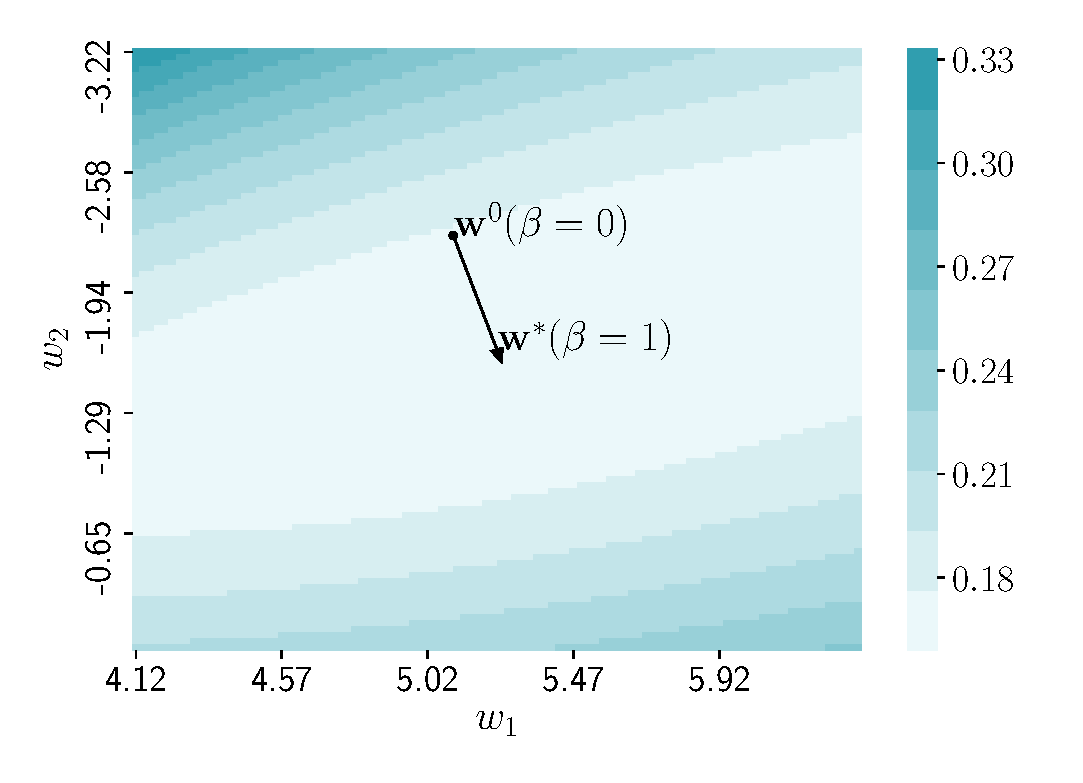
\includegraphics[width=\linewidth]{figs/ch3/log_reg_error}
		\caption{Ландшафт функции ошибки для логистической регрессии}
		\label{fig:log_reg_error}
	\end{minipage}%
	\begin{minipage}{.47\textwidth}
		\centering
		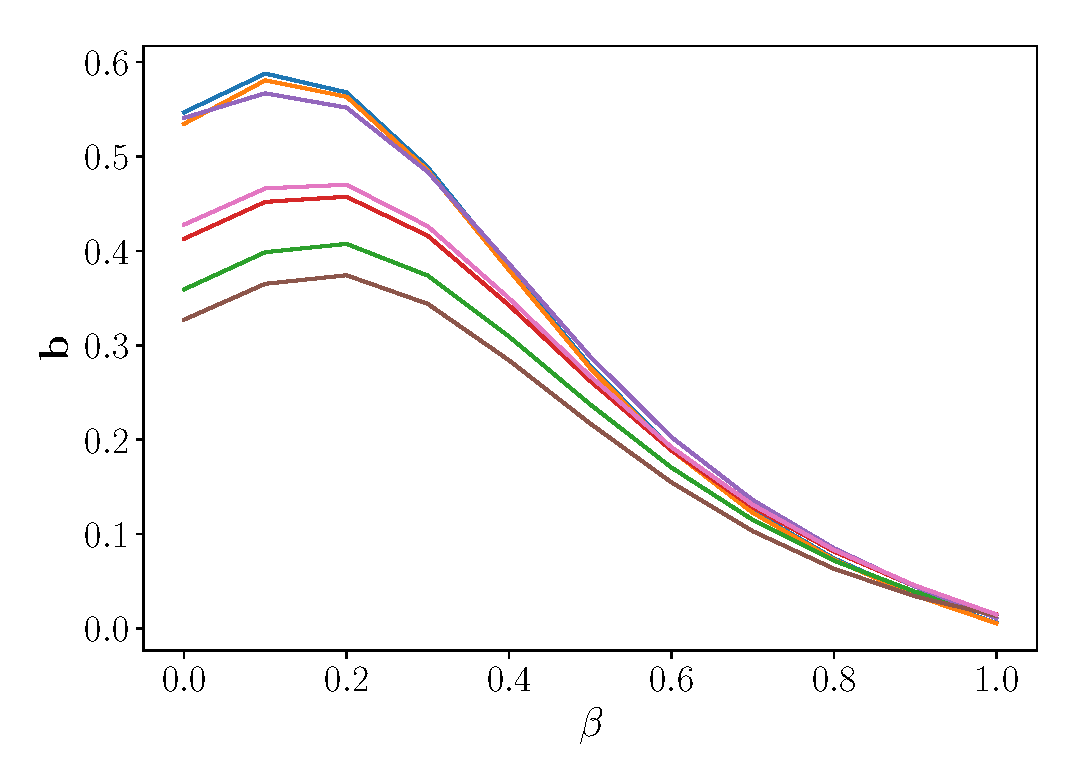
\includegraphics[width=\linewidth]{figs/ch3/log_reg_b_wrt_beta}
		\caption{Релевантности параметров для логистической регрессии}
		\label{fig:log_reg_b_wrt_beta}
	\end{minipage}
\end{figure}

Для модели нелинейной регрессии используется классический набор данных Boston Housing с 506 объектами и 13 признаками.
Для простоты нейронная сеть содержит два скрытых нейрона.
Ландшафт функции ошибок для модели нейронной сети является более сложным. 
Он не выпуклый и может содержать несколько локальных минимумов.
Двумерный ландшафт функции ошибок для этого набора данных показан на рис.~\ref{fig:neural_error}. 
Сетка строится для двух случайных весов из матрицы~$\bW_1$.
Мы используем ту же стратегию для исследования того, как вектор~$\bb$ изменяется от~$\bw^0$ до~$\bw^*$. 
Результат показан на рис.~\ref{fig:neural_b_wrt_beta}.
Компоненты вектора $\bb$ становятся близки к нулю вблизи оптимума. 
При достижении оптимального значения различные веса влияют на остатки модели~$\bz$.
\begin{figure}
	\centering
	\begin{minipage}{.5\textwidth}
		\centering
		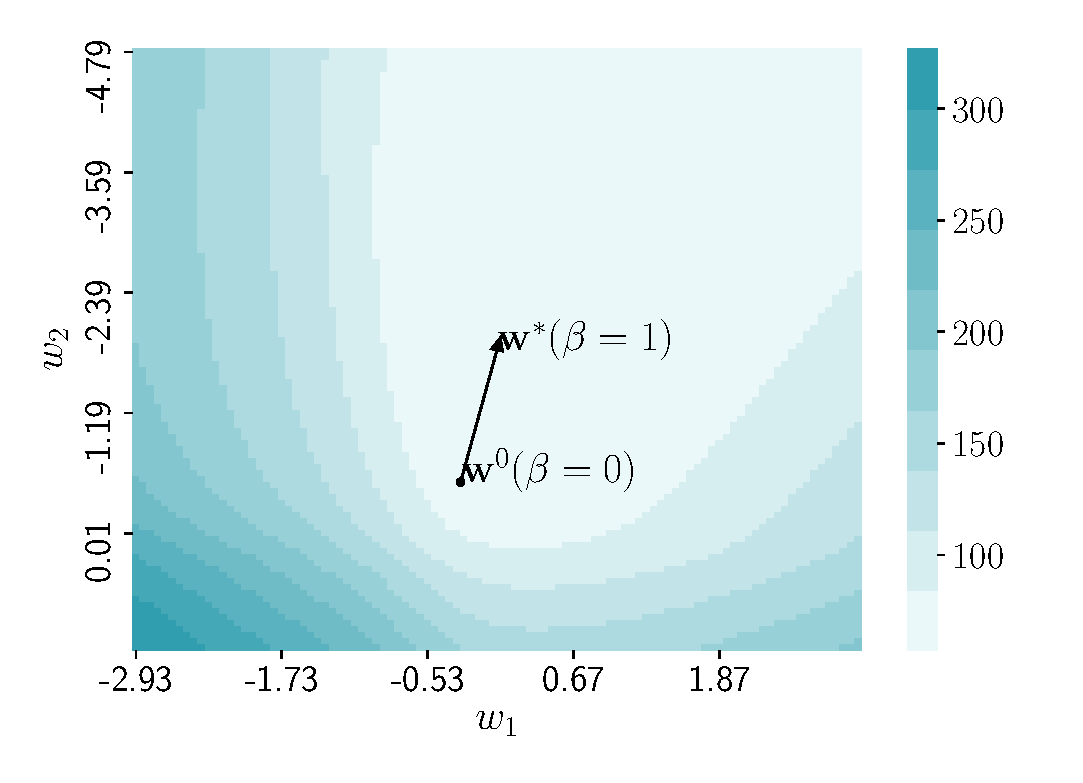
\includegraphics[width=\linewidth]{figs/ch3/neural_error}
		\caption{Ландшафт функции ошибки для нейронной сети}
		\label{fig:neural_error}
	\end{minipage}%
	\begin{minipage}{.5\textwidth}
		\centering
		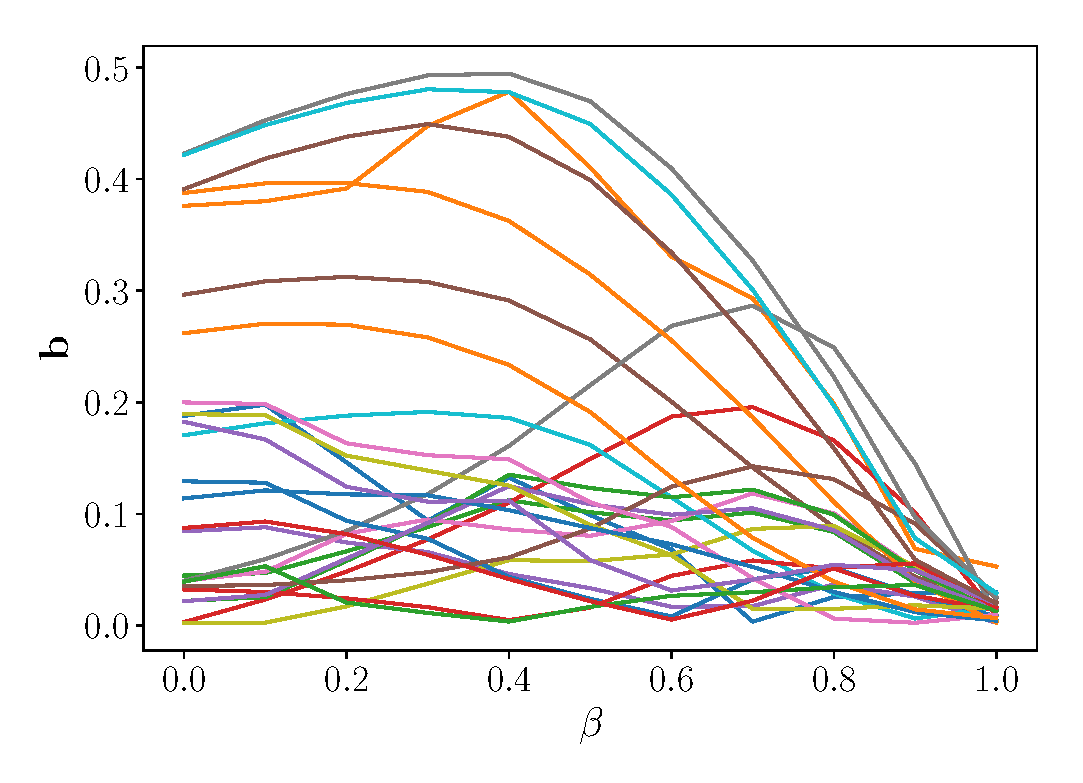
\includegraphics[width=\linewidth]{figs/ch3/neural_b_wrt_beta}
		\caption{Релевантности параметров первого слоя для модели нейронной сети}
		\label{fig:neural_b_wrt_beta}
	\end{minipage}
\end{figure}

На рис.~\ref{fig:irls_qpfs_2d} показан процесс оптимизации для предложенного алгоритма в случае логистической регрессии с двумя параметрами модели. 
Даже для двумерной задачи решение метода Ньютона нестабильно и число обусловленности матрицы Гессиана~$\bH$ может быть чрезвычайно большим. 
На каждом шаге алгоритма процедура QPFS выбирает параметры для оптимизации. 
В данном примере предложенный алгоритм выбирает и обновляет только один параметр на каждой итерации на первых шагах. 
Это делает алгоритм более устойчивым.

\begin{figure}[!ht]
	\centering
	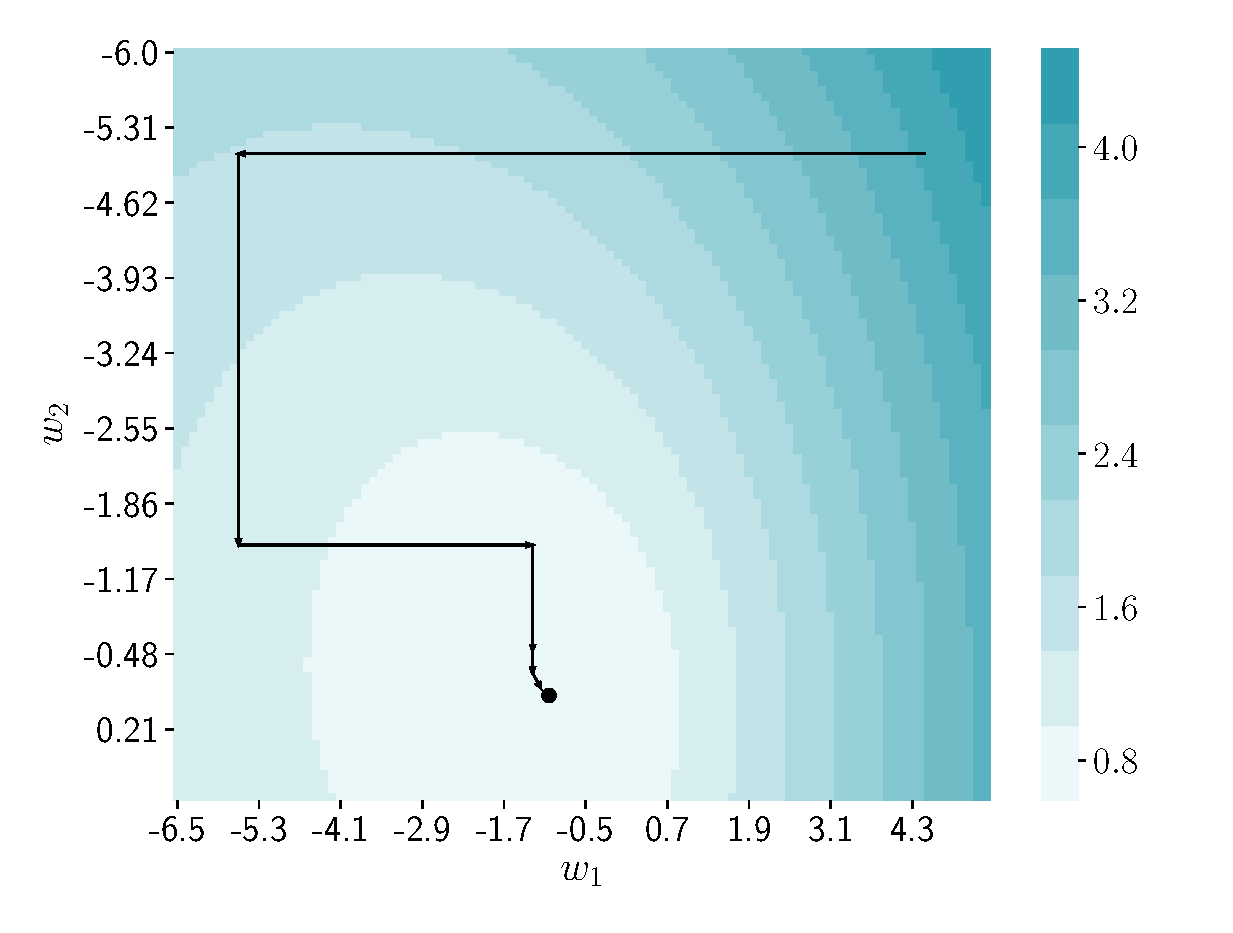
\includegraphics[width=0.6\linewidth]{figs/ch3/irls_qpfs_2d}	 
	\caption{Оптимизационный процесс предложенного алгоритма QPFS+Ньютон для модели логистической регрессии}
	\label{fig:irls_qpfs_2d}
\end{figure}

На рис.~\ref{fig:active_params_wrt_iters} показаны наборы активных параметров на итерациях для набора данных Boston Housing и нейронной сети с двумя скрытыми нейронами. 
Темные ячейки соответствуют активным параметрам, которые мы оптимизируем.

\begin{figure}[!ht]
	\centering
	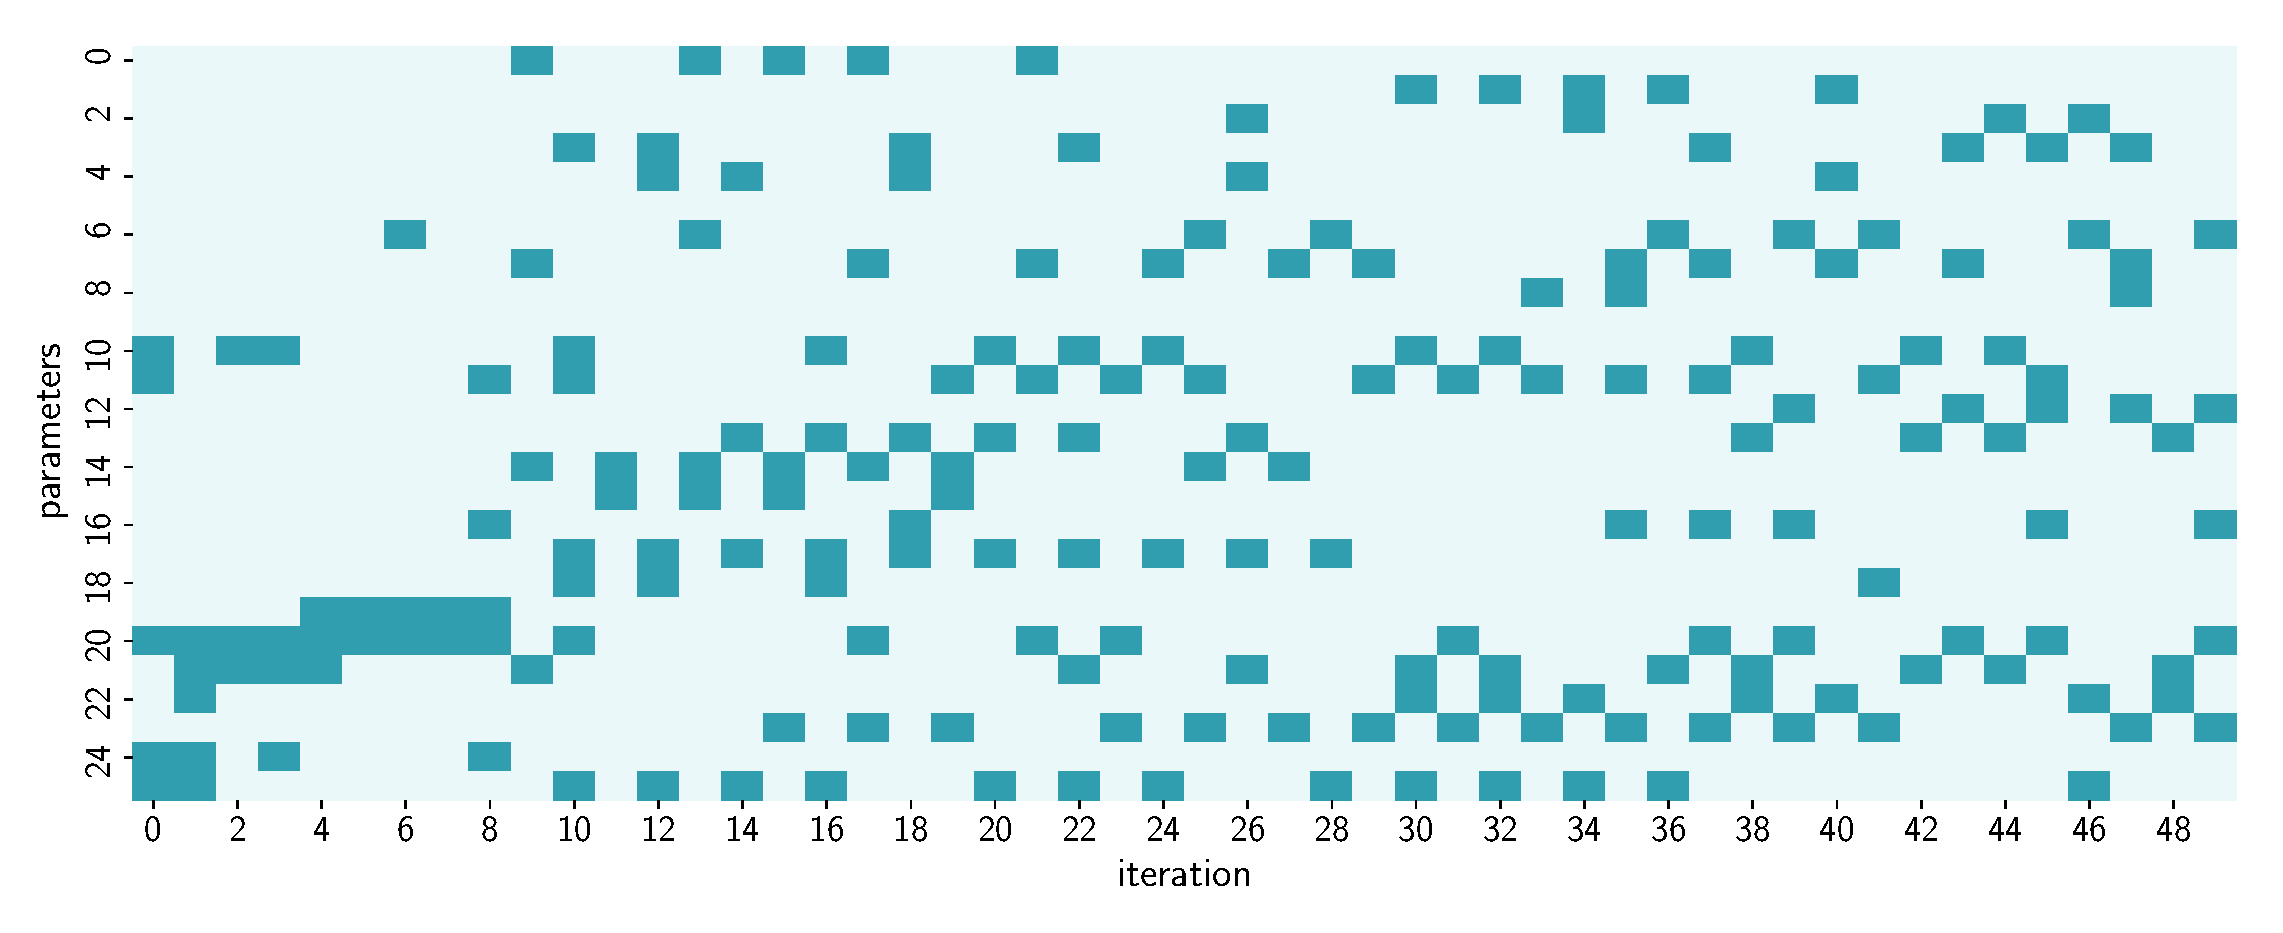
\includegraphics[width=\linewidth]{figs/ch3/active_params_wrt_iters}	
	\caption{Множества активных параметров на протяжении оптимизационного процесса}
	\label{fig:active_params_wrt_iters}
\end{figure}

В рассмотренных примерах число обусловленности~$\kappa(\bH)$ для метода Ньютона на некоторых итерациях было чрезвычайно большим. 
Выбор активных параметров позволил значительно сократить число обусловленности. 

Мы сравнили предложенный алгоритм с существующими методами, а именно градиентным спуском~(GD), моментом Нестерова, Adam и оригинальным алгоритмом Ньютона. 
Проведены эксперименты для моделей нелинейной и логистической регрессий. 
Наборы данных были выбраны из репозитория UCI~\cite{uci2017}. 
Результаты показаны в таблицах~\ref{tbl:nonlin_reg_results} и \ref{tbl:log_reg_results}. 
Для каждого набора данных две строки содержат ошибки для тренировочной~(первая строка) и тестовой~(вторая строка) выборок. 
В таблице~\ref{tbl:nonlin_reg_results} приведена квадратичная ошибка, в таблице~\ref{tbl:log_reg_results}~-- кросс-энтропия.
Чтобы найти среднюю ошибку и ее стандартное отклонение использовалась процедура кросс валидации на 5 фолдов. 
Предложенный алгоритм показывает меньшую ошибку на трех из четырех наборов данных для нелинейной регрессии и среди двух из трех наборов данных для логистической регрессии.

\begin{table}[!ht]
\footnotesize
	\caption{Средняя квадратичная ошибка на тренировочной и тестовой выборках для модели нелинейной регрессии}
	\label{tbl:nonlin_reg_results}
	\centering
	\begin{tabular}{|l|c|c|c|c|c|c|}
		\hline
		Выборка & \begin{tabular}[c]{@{}c@{}}\ $m$ \\ \ $n$ \end{tabular} 
		& GD 
		& Нестеров 
		& ADAM 
		& Ньютон 
		&
		\begin{tabular}[c]{@{}c@{}}QPFS+Ньютон\\ \end{tabular} \\ 
		\hline
		Boston House
		& 506
		& $27.2\pm4.6$
		& $46.0\pm11.0$
		& $35.4\pm2.5$           
		& $22.1\pm15.2$            
		& $20.9\pm10.4$   \\  
		Prices
		&\multicolumn{1}{c|}{13}
		& \multicolumn{1}{c|}{$32.4\pm5.6$}
		& \multicolumn{1}{c|}{$53.3\pm11.5$}
		& \multicolumn{1}{c|}{$37.8\pm7.0$}
		& \multicolumn{1}{c|}{$28.9\pm13.6$}
		& \multicolumn{1}{c|}{$\mathbf{24.5\pm9.4}$}\\ 
		\hline
		Communities
		& 1994
		& $48.0\pm6.4$
		& $31.4\pm2.8$
		& $23.3\pm3.7$        
		& $18.3\pm3.4$          
		&  $26.7\pm3.1$  \\ 
		and Crime
		&\multicolumn{1}{c|}{99}
		& \multicolumn{1}{c|}{$47,5\pm6.5$}
		& \multicolumn{1}{c|}{$32.9\pm4.3$}
		& \multicolumn{1}{c|}{$28,1\pm4.5$}
		& \multicolumn{1}{c|}{$28.8\pm3.6$}
		& \multicolumn{1}{c|}{$\mathbf{28.4\pm3.0}$} \\ 
		\hline
		Forest
		& 517
		& $18.9\pm0.4$
		& $1.83\pm0.4$
		& $1.81\pm0.6$             
		& $17.7\pm0.4$             
		& $17.9\pm0.4$   \\ 
		Fires
		&\multicolumn{1}{c|}{10}
		& \multicolumn{1}{c|}{$\mathbf{20.0\pm2.1}$}
		& \multicolumn{1}{c|}{ $20.2\pm2.2$}
		& \multicolumn{1}{c|}{ $\mathbf{20.0\pm2.0}$}
		& \multicolumn{1}{c|}{ $20.6\pm1.4$}
		& \multicolumn{1}{c|}{ $20.2\pm2.2$} \\ 
		\hline
		Residential
		& 372
		&  $51.6\pm17.7$
		&  $32.6\pm19.5$
		&  $30.0\pm24.8$            
		&  $35.5\pm24.7$            
		&   $30.3\pm10.7$ \\ 
		Building
		&\multicolumn{1}{c|}{103}
		& \multicolumn{1}{c|}{ $53.7\pm13.9$}
		& \multicolumn{1}{c|}{ $34.1\pm13.6$}
		& \multicolumn{1}{c|}{ $34.1\pm19.4$}
		& \multicolumn{1}{c|}{ $35.0\pm15.6$}
		& \multicolumn{1}{c|}{ $\mathbf{30.9\pm5.3}$} \\ 
		\hline
	\end{tabular}
\end{table}

\begin{table}[!ht]
\footnotesize
	\caption{Среднее значение кросс-энтропии на тренировочной и тестовой выборках для модели логистической регрессии}
	\label{tbl:log_reg_results}
	\centering
	\begin{tabular}{|l|c|c|c|c|c|c|}
		\hline
		Выборка & \begin{tabular}[c]{@{}c@{}}\ $m$ \\ \ $n$ \end{tabular} 
		& GD 
		& Нестеров 
		& ADAM 
		& Ньютон 
		&
		\begin{tabular}[c]{@{}c@{}}QPFS+Ньютон\\ \end{tabular} \\ 
		\hline
		Breast
		& 569
		& $0.6\pm0.1$
		& $0.4\pm0.1$
		& $0.8\pm0.2$           
		& $0.3\pm0.1$            
		& $0.2\pm0.1$   \\  
		Cancer
		&\multicolumn{1}{c|}{30}
		& \multicolumn{1}{c|}{$\mathbf{0.9\pm0.2}$}
		& \multicolumn{1}{c|}{$1.0\pm0.7$}
		& \multicolumn{1}{c|}{$1.2\pm0.2$}
		& \multicolumn{1}{c|}{$1.0\pm0.2$}
		& \multicolumn{1}{c|}{$1.1\pm0.3$}\\ 
		\hline
		Cardiotocography
		& 2126
		& $11.5\pm4.7$
		& $11.5\pm4.7$
		& $8.8\pm4.4$        
		& $11.5\pm5.7$          
		&  $7.7\pm4.2$  \\
		
		&\multicolumn{1}{c|}{21}
		& \multicolumn{1}{c|}{$11.6\pm5.8$}
		& \multicolumn{1}{c|}{$11.5\pm5.7$}
		& \multicolumn{1}{c|}{$9.0\pm2.6$}
		& \multicolumn{1}{c|}{$11.5\pm4.7$}
		& \multicolumn{1}{c|}{$\mathbf{7.7\pm4.7}$} \\ 
		\hline
		Climate Model
		& 540
		& $1.2\pm0.1$
		& $1.0\pm0.2$
		& $1.5\pm0.2$             
		& $1.0\pm0.5$             
		& $0.8\pm0.3$   \\ 
		Simulation Crashes
		&\multicolumn{1}{c|}{18}
		& \multicolumn{1}{c|}{$1.4\pm2.0$}
		& \multicolumn{1}{c|}{ $1.3\pm0.7$}
		& \multicolumn{1}{c|}{ $1.8\pm0.3$}
		& \multicolumn{1}{c|}{ $1.2\pm0.5$}
		& \multicolumn{1}{c|}{ $\mathbf{1.1\pm0.4}$} \\ 
		\hline
	\end{tabular}
\end{table}

